\def\SECTION{2.5 Two-Column Proofs}
\documentclass[aspectratio=169,14pt]{beamer}
\usepackage[T1]{fontenc}
\usepackage{mathpazo}
\usepackage{amsmath,amssymb}
\usepackage{tikz}
\usetikzlibrary{arrows.meta,calc,decorations.pathreplacing}
\definecolor{fblue}{HTML}{1F4E79}
\definecolor{fteal}{HTML}{0F7C7C}
\definecolor{fgold}{HTML}{C9962B}
\definecolor{fred}{HTML}{B3261E}
\definecolor{fink}{HTML}{16233B}
\definecolor{fsoft}{HTML}{EEF3F8}
\definecolor{fgoldsoft}{HTML}{FBF1DC}
\setbeamertemplate{navigation symbols}{}
\setbeamercolor{normal text}{fg=fink}
\setbeamercolor{frametitle}{fg=fblue}
\setbeamerfont{frametitle}{series=\bfseries,size=\Large}
\setbeamercolor{structure}{fg=fteal}
\setbeamertemplate{itemize item}{\color{fteal}$\blacktriangleright$}
\setbeamertemplate{frametitle}{\vspace{6pt}\insertframetitle\par\vspace{-2pt}{\color{fgold}\rule{2.2cm}{2pt}}}
\setbeamertemplate{footline}{\hspace{0.6cm}{\color{fblue}\scriptsize\bfseries Fang\textcolor{fteal}{Math}}\hfill{\scriptsize\color{gray}\SECTION\quad\insertframenumber}\hspace{0.6cm}\vspace{6pt}}
\newcommand{\key}[1]{{\color{fteal}\textbf{#1}}}
\newcommand{\ans}[1]{\colorbox{fgoldsoft}{\color{fink}\ensuremath{#1}}}
\newcommand{\warn}[1]{\begin{beamercolorbox}[sep=8pt,rounded=true]{warnbox}{\color{fred}\textbf{Watch out!}}\enskip #1\end{beamercolorbox}}
\setbeamercolor{warnbox}{bg=fred!8,fg=fink}
\setbeamercolor{turnbox}{bg=fgoldsoft,fg=fink}
\setbeamercolor{defbox}{bg=fsoft,fg=fink}
\newcommand{\defn}[1]{\begin{beamercolorbox}[sep=8pt,rounded=true]{defbox}#1\end{beamercolorbox}}
\newenvironment{yourturn}{\begin{beamercolorbox}[sep=10pt,rounded=true]{turnbox}{\color{fgold}\Large\bfseries Your turn!}\quad{\small Pause the video and try it.}\par\medskip}{\end{beamercolorbox}}
\newcommand{\titleframe}[3]{%
\begin{frame}[plain]
\begin{tikzpicture}[remember picture,overlay]
\fill[fblue] (current page.north west) rectangle ([yshift=-0.9cm]current page.north east);
\node[anchor=west,text=white,font=\bfseries] at ([xshift=0.6cm,yshift=-0.45cm]current page.north west) {Fang\textcolor{fgold}{Math}};
\node[anchor=east,text=white,font=\small] at ([xshift=-0.6cm,yshift=-0.45cm]current page.north east) {Geometry $\cdot$ Chapter \CHNO};
\end{tikzpicture}
\vfill
{\color{fteal}\large\bfseries #1}\par\medskip
{\color{fblue}\fontsize{30}{34}\selectfont\bfseries #2}\par\medskip
{\color{fgold}\rule{3cm}{3pt}}\par\bigskip
{\large #3}
\vfill
{\small\color{gray} fangmath.com $\cdot$ YouTube @fangmathcom}
\end{frame}}
\newcommand{\closeframe}[1]{%
\begin{frame}{Remember}
#1
\vfill
\begin{center}{\color{fblue}\large\bfseries Now practice at your level:}\par\smallskip
{\Large\color{fteal}\bfseries fangmath.com} \enskip{\color{gray}$\to$ Geometry $\to$ Chapter \CHNO}\end{center}
\end{frame}}

\usepackage{pgfplots}\pgfplotsset{compat=1.17}
\newcommand{\grid}[4]{\draw[step=1,gray!25] (#1,#2) grid (#3,#4);\draw[-{Stealth},gray] (#1,0)--(#3+0.3,0) node[right]{\small$x$};\draw[-{Stealth},gray] (0,#2)--(0,#4+0.3) node[above]{\small$y$};}
\def\CHNO{2}
\usetikzlibrary{angles,quotes}
\begin{document}
\titleframe{Lesson 2.5}{Two-Column Proofs}{Statements on the left, reasons on the right}
\begin{frame}{What a two-column proof looks like}
\onslide<1->{\begin{tabular}{l|l}\textbf{Statements} & \textbf{Reasons}\\ \hline 1.\ \ldots\ (given) & Given\\ 2.\ \ldots & a property, definition, \ldots\\ \ldots\ (what you must prove) & \ldots\end{tabular}}\par\medskip
\onslide<2->{\defn{Start with what is \key{given}. End with what you must \key{prove}. Every line must follow from the lines above it.}}\par\medskip
\end{frame}
\begin{frame}{An algebra proof}
\onslide<1->{Given: $2x + 5 = 13$ \qquad Prove: $x = 4$}\par\medskip
\onslide<2->{1.\ $2x + 5 = 13$ \hfill Given}\par\medskip
\onslide<3->{2.\ $2x = 8$ \hfill Subtraction Property of Equality}\par\medskip
\onslide<4->{3.\ $x = 4$ \hfill Division Property of Equality}\par\medskip
\end{frame}
\begin{frame}{A geometry proof}
\begin{columns}[c]\begin{column}{0.44\textwidth}\centering 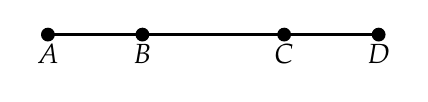
\begin{tikzpicture}\draw[very thick] (0,0)--(4.2,0); \foreach \x/\l in {0/A,1.2/B,3/C,4.2/D} \fill (\x,0) circle(2.5pt) node[below]{$\l$};\end{tikzpicture}\end{column}\begin{column}{0.54\textwidth}\onslide<1->{Given: $AB = CD$ \qquad Prove: $AC = BD$}\par\medskip
\onslide<2->{1.\ $AB = CD$ \hfill Given \\ 2.\ $BC = BC$ \hfill Reflexive Property}\par\medskip
\onslide<3->{3.\ $AB + BC = BC + CD$ \hfill Addition Property of Equality}\par\medskip
\onslide<4->{4.\ $AB + BC = AC$, \ $BC + CD = BD$ \hfill Segment Addition Postulate}\par\medskip
\onslide<5->{5.\ $AC = BD$ \hfill Substitution Property}\par\medskip\end{column}\end{columns}
\end{frame}
\begin{frame}{Watch out}
\onslide<1->{\warn{A reason must be a \textbf{given}, a \textbf{definition}, a \textbf{property}, a \textbf{postulate} or a \textbf{theorem} --- never ``it looks like it'' or ``I calculated it''.}}\par\medskip
\end{frame}
\begin{frame}{}
\begin{yourturn}Given: $5x - 2 = 18$ \quad Prove: $x = 4$ \\ 1.\ $5x - 2 = 18$ \ Given \quad 2.\ $5x = 20$ \ \underline{\ ?\ } \quad 3.\ $x = 4$ \ \underline{\ ?\ }\end{yourturn}\par\medskip
\onslide<2->{2.\ \ans{\text{Addition Property of Equality}} \quad 3.\ \ans{\text{Division Property of Equality}}}\par\medskip
\end{frame}
\closeframe{\begin{itemize}\setlength\itemsep{8pt}
\item \key{Statements} on the left, \key{reasons} on the right.
\item Start with the \key{given}; end with what you must \key{prove}.
\item Every reason is a given, definition, property, postulate or theorem.
\end{itemize}}
\end{document}
